% * * * * * * * * * * * * * * * * * * * * * * * * * * * * * * * * * * *
% *                             Thesis                                *
% *                 https://github.com/Jacopx/Thesis                  *
% * * * * * * * * * * * * * * * * * * * * * * * * * * * * * * * * * * *

\documentclass[%
    corpo=12pt,
    twoside,
%    stile=classica,
    oldstyle,
    autoretitolo,
    greek,
    evenboxes,
%    tipotesi,
]{toptesi}
%%%%%%%%%%%%%%%%%%%%%%%%%%%%%%%%%%%%%%%%%%%%%%%%%%%%

\usepackage[utf8]{inputenc}
\usepackage[T1]{fontenc}
\usepackage{lmodern}
\usepackage{hyperref}
\usepackage{graphicx}
\usepackage{subfigure}
\usepackage{booktabs}
\usepackage{amsfonts}
\usepackage{amssymb}
\usepackage{bm}
\usepackage{listings}

\hypersetup{%
    pdfpagemode={UseOutlines},
    bookmarksopen,
    pdfstartview={FitH},
    colorlinks,
    linkcolor={blue},
    citecolor={blue},
    urlcolor={blue}
  }

%%%%%%% Definizioni locali
\newtheorem{osservazione}{Osservazione}% Standard LaTeX


\begin{document}

\ateneo{Politecnico di Torino}
%
% Non tutte le università hanno un nome proprio
%\nomeateneo{Sede di Torre Elettra}
%
% \FacoltaDi{Faculty of Computer Engineering}% lo spazio finale correttamente sparisce

\titolo{Time  prediction of software development via machine learning}
\sottotitolo{Artificial Intelligence applied to Software Engineering}

%
%%%%%%% Corso degli studi
\corsodilaurea{Computer Engineering}% per la laurea
%\corsodidottorato{Meccanica}% per il dottorato

\renewcommand*\IDlabel{}
%
\candidato{Jacopo \textsc{Nasi} [255320]}

%%%%%%% Relatori o supervisori
\relatore{prof.~Maurizio Morisio}

%%%%%%% Tutore
\tutoreaziendale{dott.\ Davide Piagneri}
\NomeTutoreAziendale{Supervisore aziendale\\EisWORLD SRL}

\sedutadilaurea{\textsc{Anno~accademico} 2019-2020}


%%%%%%% Logo della sede
\logosede{polito}

%%%%%%% OFFSET
%\setbindingcorrection{3mm}

\english%  di default e' in vigore \italiano

\iflanguage{english}{%
	\retrofrontespizio{This work is subject to the Creative Commons Licence}
	\DottoratoIn{PhD Course in\space}
	\CorsoDiLaureaIn{Master degree course in\space}
	\NomeMonografia{Bachelor Degree Final Work}
	\TesiDiLaurea{Master Degree Thesis}
	\NomeDissertazione{PhD Dissertation}
	\InName{in}
	\CandidateName{Candidates}% or Candidate
	\AdvisorName{Supervisors}% or Supervisor
	\TutorName{Tutor}
	\NomeTutoreAziendale{Internship Tutor}
	\CycleName{cycle}
	\NomePrimoTomo{First volume}
	\NomeSecondoTomo{Second Volume}
	\NomeTerzoTomo{Third Volume}
	\NomeQuartoTomo{Fourth Volume}
	\logosede{polito}% or comma separated list of logos
}{}
%%%%%%%%%%%%%%%%%%%%%%%%%%%%%%%%%%%%%%%%%

\frontespizio

\summary

La pressione barometrica di Giove viene misurata
mediante un metodo originale  messo a punto dai candidati, che si basa
sul rilevamento telescopico della pressione.

% \paginavuota % funziona anche senza specificare l'opzione classica

\acknowledgements

Un ringraziamento speciale ai cavalieri di Smirnuff, luce della mia battaglia.

\indici

\mainmatter

% #######################################
% #            Introduction             #
% #######################################

\chapter{Introduction}

\section{General Problem}
Forecasting is one of the most critic part of a company, it could drive to easily success as well as drive to failure. A software project is not different from a manufacturing product, its development, infact, require analysis of different kind, from resources needed to costs and time required.\\
The software development experience shows that the process of analysis is really difficult, due to the nature of the problem, coding is a mind product and the time required to produce it can varying in accord to a lot of different factors.

\section{Tools used}
This work is mainly conducted using software tools, here a list of the tools used:

\paragraph{\href{https://www.python.org/}{Python}} The main programming language of the thesis project. Used for data management, feature extraction, machine learning models and for interfaction with other softwares. The specific version used is the v3.7.0

\paragraph{\href{https://pandas.pydata.org/}{Pandas}} Open source, BSD-licensed library providing high-performance, easy-to-use data structures and data analysis tools for the Python programming language.

\paragraph{\href{https://numpy.org/}{NumPy}} Scientific computing with Python.

\paragraph{\href{https://matplotlib.org/}{Matplotlib}} 2D Plotting library for Python.

\paragraph{\href{https://seaborn.pydata.org/}{Seaborn}} Another plotting library for Python.

\paragraph{\href{https://www.tensorflow.org/}{Tensorflow}} Platform for machine learning.

\paragraph{\href{https://keras.io/}{Keras}} High level API for neural networks.

\paragraph{\href{https://scikit-learn.org/stable/}{SciKit-Learn}} Tools and libraries for machine learning.

\paragraph{\href{https://gitlab.com}{GitLab}} Sourcing platform based on Git. Used for the code of the project, available here:\\
\url{https://gitlab.com/EiS-Projects/analytics/temp/thesisProjectJN}.

\paragraph{\href{https://github.com}{GitHub}} Sourcing platform based on Git. Used for the thesis and calendar sourcing:
\begin{itemize}
  \item Thesis: \url{https://github.com/Jacopx/Thesis}
  \item Calendar: \url{https://github.com/Jacopx/ThesisCalendar}
\end{itemize}

\paragraph{\href{https://www.jetbrains.com/}{JetBrains IDEs}} Student-free IDE for different language development, product used:
\begin{itemize}
  \item PyCharm: \url{https://www.jetbrains.com/pycharm/}
  \item DataGrip: \url{https://www.jetbrains.com/datagrip/}
\end{itemize}

% #######################################
% #              Datasets               #
% #######################################

\chapter{Datasets}
The following section illustrate the structure of the all the principal datasets used during this thesis project.
\section{SEOSS33}
The SEOSS33\cite{SEOSS33} is a \href{https://doi.org/10.7910/DVN/PDDZ4Q}{dataset} collecting bug, issue, reports, commit and lot of other information of 33 open source project, following their progress via sourcing platform. At today there are no other public research conducted over this datasets, this works seems to be first.\\
Is fundamental to understand the structure of this dataset, the majority of the forecasting operation tests are conducted using the data stored by this research.\\
Each project is stored in a SQLITE db file, a SQL offline database, the structure is based on the entity of the \textit{issue}, identified by an \textit{issue\_id}, the other tables are used to link additional information, like the number of commit, the version referred, comments and others features. The figure \ref{fig:seoss33_db} show the database schema.

\begin{figure}[!h]
  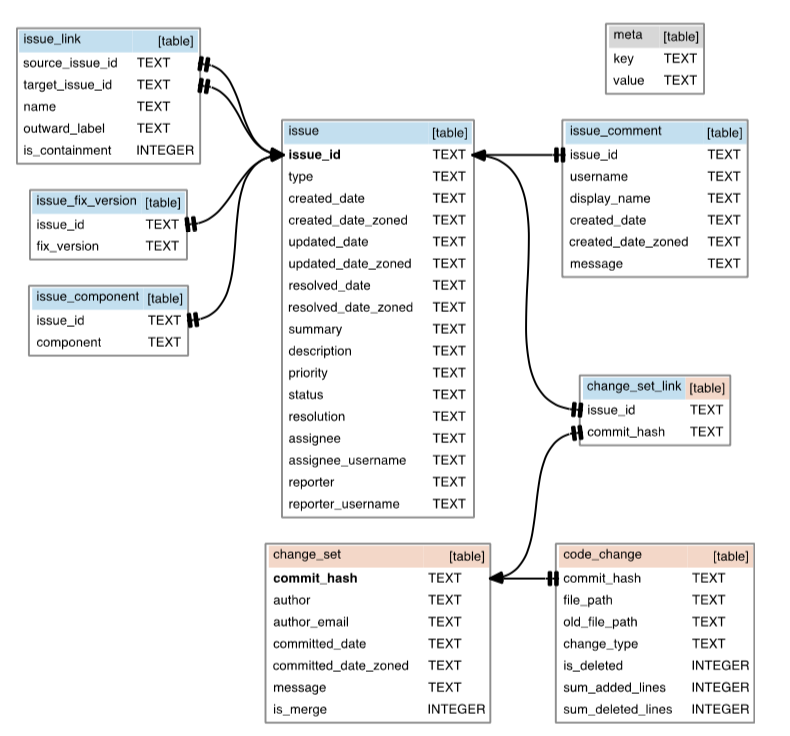
\includegraphics[width=\linewidth]{figure/seoss33_db_schema.png}
  \caption{SEOSS33 data model}
  \label{fig:seoss33_db}
\end{figure}

The dataset is composed of 33 different software projects with some common characteristics (reference in  \cite{SEOSS33} chapter 2.1), almost single programming language (Java), usage of versioning software, tracebility of issue and other similiar information. Among these products we have selected five of them, because of size, as shown in table \ref{tab:seoss33_selected}:

\begin{center}
  \captionof{table}{Project data distribution} \label{tab:seoss33_selected}
  \begin{tabular}{ |c|c|c| }
     \hline
     \textbf{Project} & \textbf{Month} & \textbf{Issue} \\
     \hline
     \hline
     Hadoop & 150 & $39086$ \\
     Hbase & 131 & $19247$ \\
     Maven & 183 & $18025$ \\
     Cassandra & 106 & $13965$ \\
     Hive & 113 & $18025$ \\
     \hline
  \end{tabular}
\end{center}


% \section{San Francisco Bike Sharing}
% The big US city of San Francisco provide a lot of public available dataset related to the service proposed, one of them is about the BS (\textit{Bike Sharing}) system of the Bay Area. It's a huge \href{https://www.kaggle.com/datasf/san-francisco}{dataset} holding information about 5 years, for 70 stations, with more than 5000 bikes.
% The structure is simple and is divided among three tables:
% \begin{itemize}
%   \item \textbf{status}: A log storing the information of number of bikes and docks available at each minute of the day for each station
%   \item \textbf{trips}: Each ride performed with the source and destination station, the starting and arrival time, the duration, the number of the bike used and the type of user subscription.
%   \item \textbf{stations}: Store generical informations about the station, name, address, latitude, longitude and number of docks.
% \end{itemize}
%
% \section{San Francisco Fire Department}
% Another dataset, of the city of San Francisco, available is related to the fire department. The dataset is based on a \href{https://data.sfgov.org/widgets/nuek-vuh3}{big table} where each row is referring to a unit dispatched, \textit{Unit ID} for an operations, more than one unit can be involved in a single operations that can be identified by the field \textit{call number}. Many others features can be found in the remaining fields, operations GPS location, type of allarm, type of operation.


% #######################################
% #          Machine Learning           #
% #######################################

\chapter{Machine Learning models}
\section{Introduction}
Machine learning (ML) is the scientific study of algorithms and statistical models that computer systems use to perform a specific task without using explicit instructions, relying on patterns and inference instead\cite{ml}. The word ML is almost in the public domain now, in the last decades the usage of these kind of algorithms has drammatically raisen although most of it had already been developed for years. The main reason is the increase in the computational capacity of the systems.\\
There a lot of different models available, the following chapters will focus on the models used in this project.

\section{Random Forest}
Random Forest (RF) is a supervised Learning algorithm which uses ensemble learning method for classification and regression. The forest is made by lot of different decision tree, its basic unit. The structure of the decision tree is simple, each branch define a direction to follow based on the values of different features, the end of a branch, the leaf, instead is the final predicted value. When all the trees are trained the model can be used, all the features value are evaluated by all the trees, than using some aggregation technique the final predicted value is computed. Using lot of different decision tree reduce the habit of overfitting. The behaviour is similar even for classification. Figure \ref{fig:rf} shows a simplified schema of the model.
\begin{figure}[!h]
  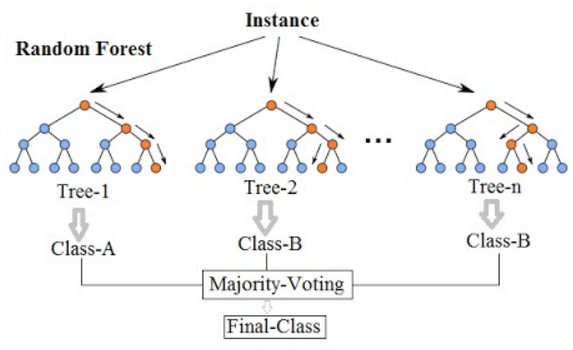
\includegraphics[width=\linewidth]{figure/rf.png}
  \caption{Random Forest simplified scheme \cite{rf}}
  \label{fig:rf}
\end{figure}

The main advantages are that is efficent on large databases, can handle a lot of input variables without variable deletion, it generate an unbiased estimate of the generalization error for the build process and it can handle missing data.
One of the drawback of this technique is the habit to overfit in particular condition, depending on datasets.


\section{Neural Networks}
Neural Networks (NN) are algorithm, for pattern recognition, inspired by the structure of the human brain, with elaboration units (neurons) and connection network (synapses), exposed to enough of the right data, this kind of algorithms is able to establish correlations between present and future events. Figure \ref{fig:nn} shows a simplyfied versiona of a neural network.\\
NN can be used to solve different kind of problems, classification, clustering and regression. Our problem will be solved using the regressive type.\\
Regression analysis can be used to forecast one or more label based to other features.
\begin{figure}[!h]
  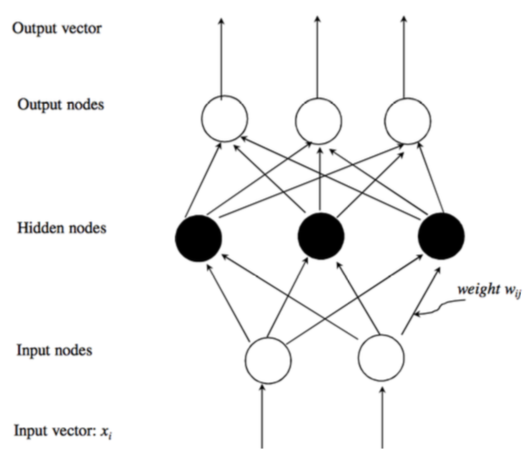
\includegraphics[width=\linewidth]{figure/nn.png}
  \caption{Structure of a neural network}
  \label{fig:nn}
\end{figure}
The structure of these networks can be really complicated and a whole thesis can be made upon this topic that, for this reason, will not more discussed.

\paragraph{Recurrent Neural Networks}
Recurrent Neural Networks (RNN) is a class of NN that keep connections between nodes and a temporal sequence. The main difference, respect NN, is that has feedback connections, this memory allow to keep track of temporal dynamic behaviour, they can process single data point or entire sequence of data, like video or speech.

\paragraph{Long-Short Term Memory}
One of the most used type of RNN is the Long-Short Term Memory (LSTM), were developed to solve the problems of exploding and vanishing of gradient typical of normal RNN.


% #######################################
% #             Forecasting             #
% #######################################

\chapter{Forecasting}
\section{Introduction}
Forecasting is the process of making predictions of future based on past and present data by trends analysis. Forecasting is one of the most desired machine learning functionality, it could be used to improve each kind of process, from finacials to production ones. Of course this task is not easy to achieve, a lot of resources and studies are needed to accomplish it.
The software development is identical to a product development process, starts from the ideation and ends with the production itself.
The goal is to predict the defectiveness in order to efficently allocate the development effort.

\section{Features}
The main advantage, in data analysis, of machines is that they can compute a lot of different data and finding a lot of patterns and correlation that human can't find. Combine the human attitude of logical correlations and machines capacity of number analysis can drive to a powerful combination that can drastically improve the forecasting ability.
Each artificial intelligence algorithms require a correct and properly studied data in order to perform a valuable prediction, one of the basic step is the data preparation, providing correct and organized data is fundamental to correctly fit the network over the problem.

\section{Models detail}
\section{One-Shot Prediction}
\section{Recurrent forecasting}
\section{Results}


% % #######################################
% % #         Model abstraction           #
% % #######################################
%
% \chapter{Model abstraction}
% % \section{CommonDB}
% \section{SFBS and literature comparisons}
% \section{SFFD}


% #######################################
% #             Conclusion              #
% #######################################

\chapter{Conclusion}



% #######################################
% #            BIBLIOGRAPHY             #
% #######################################
\bibliography{biblio}
\bibliographystyle{QUICKtran}

\end{document}
